%\documentclass[mathserif]{beamer}
\documentclass[handout]{beamer}
%\usetheme{Goettingen}
\usetheme{Warsaw}
%\usetheme{Singapore}
%\usetheme{Frankfurt}
%\usetheme{Copenhagen}
%\usetheme{Szeged}
%\usetheme{Montpellier}
%\usetheme{CambridgeUS}
%\usecolortheme{}
%\setbeamercovered{transparent}
\usepackage[english, activeacute]{babel}
\usepackage[utf8]{inputenc}
\usepackage{amsmath, amssymb}
\usepackage{dsfont}
\usepackage{graphics}
\usepackage{cases}
\usepackage{graphicx}
\usepackage{pgf}
\usepackage{epsfig}
\usepackage{amssymb}
\usepackage{multirow}	
\usepackage{amstext}
\usepackage[ruled,vlined,lined]{algorithm2e}
\usepackage{amsmath}
\usepackage{epic}
\usepackage{epsfig}
\usepackage{fontenc}
\usepackage{framed,color}
\usepackage{palatino, url, multicol}
\usepackage{listings}
%\algsetup{indent=2em}


\vspace{-0.5cm}
\title{Bayesian Linear Models}
\vspace{-0.5cm}
\author[Felipe Bravo Márquez]{\footnotesize
%\author{\footnotesize  
 \textcolor[rgb]{0.00,0.00,1.00}{Felipe José Bravo Márquez}} 
\date{ \today }




\begin{document}
\begin{frame}
\titlepage


\end{frame}


%%%%%%%%%%%%%%%%%%%%%%%%%%%


\begin{frame}{Bayesian Linear Models}
\scriptsize{
\begin{itemize}
\item In this class we are going to revisit the linear regression model from a Bayesian point of view.

\item The idea is the same as in the frequentist approach, to model the relationship of a numerical dependent variable $\mathbf{y}$ with $n$ independent variables  $\mathbf{x}_1, \mathbf{x}_2, \dots, \mathbf{x}_n$.

\item We again use  a Gaussian distribution to describe our  uncertainty about the response variable: $y_i \sim N(\mu_i, \sigma^2)$.

\item And we also assume that each attribute has a linear relationship to the mean of the outcome.

\begin{displaymath}
\mu_i = \beta_0 + \beta_1 x_i + \dots \beta_n x_n
\end{displaymath}

\item Instead of using least squares or maximum likelihood estimation we are going to estimate the joint posterior distribution of all the parameters of the model:

\begin{displaymath}
f(\theta|d)= f(\beta_0,\beta_1,\dots,\beta_n,\sigma|d)
\end{displaymath}


\item This approach is more flexible as it allows incorporating prior information.

\item It also allows to interpret the uncertainty of the model in a clearer way.




 
\end{itemize}



} 

\end{frame}



\begin{frame}{Bayesian Linear Models}
\scriptsize{
\begin{itemize}


\item Notice the the parameters of the model are $\beta_0,\beta_1,\dots,\beta_b$ and $\sigma$.

\item The mean of the outcome $\mu_i$ is not treated as parameter because it is determined deterministically from the linear model's coefficients.

\item To complete the model, we need a joint prior density:

\begin{displaymath}
f(\theta)= f(\beta_0,\beta_1,\dots,\beta_n,\sigma)
\end{displaymath}

\item And the posterior gets specified as follows:

\begin{displaymath}
f(\theta|d)= \frac{ \prod_{i=1}^m f(d_i|\beta_0,\beta_1,\cdots,\beta_n,\sigma)*f(\beta_0,\beta_1,\dots,\beta_n,\sigma)}{f(d)}
\end{displaymath}


here $d_i$ corresponds to each data point containing values for $y$ and $x_1,\dots,x_n$.







 
\end{itemize}



} 

\end{frame}



\begin{frame}{Bayesian Linear Models}
\scriptsize{
\begin{itemize}


\item The evidence is expressed by a multiple integral:

\begin{displaymath}
 f(d) = \int \int \dots \int \prod_{i=1}^m f(d_i|\beta_0,\beta_1,\cdots,\beta_n,\sigma)* f(\beta_0,\beta_1,\dots,\beta_n,\sigma) d\beta_0 d\beta_1 \cdots d\beta_nd\sigma
\end{displaymath}



\item In most cases, priors are specified independently for each parameter, which amounts to assuming:


\begin{displaymath}
f(\beta_0,\beta_1,\cdots,\beta_b,\sigma)=f(\beta_0)*f(\beta_1)*\dots*f(\beta_n)*f(\sigma). 
\end{displaymath}



\item This class is based on chapters 4 and 5 of \cite{mcelreath2020statistical}



 
\end{itemize}



} 

\end{frame}



\begin{frame}[fragile]{A model of height revisited}
\scriptsize{
\begin{itemize}
 \item  Let's fit again a linear model relating height and weight for the !Kung San people.
 
 \item But his time we will use a Bayesian approach.
 
 \item We need to define a probabilistic model specifying all the components of the Bayesian model:
 
 \begin{figure}[h!]
	\centering
	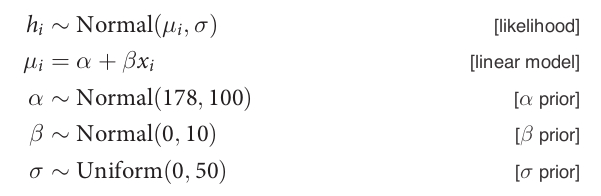
\includegraphics[scale=0.4]{pics/height_model.png}
\end{figure}
 
\end{itemize}
 

 
}
\end{frame}

\begin{frame}{Conclusions}
\scriptsize{

\begin{itemize}
\item Blabla
\end{itemize}


} 
\end{frame}


%%%%%%%%%%%%%%%%%%%%%%%%%%%
\begin{frame}[allowframebreaks]\scriptsize
\frametitle{References}
\bibliography{bio}
\bibliographystyle{apalike}
%\bibliographystyle{flexbib}
\end{frame}  









%%%%%%%%%%%%%%%%%%%%%%%%%%%

\end{document}
